\documentclass[runningheads]{llncs}
\usepackage[utf8]{inputenc}
\usepackage[T1]{fontenc}
\def\figurename{Figura}\def\tablename{Tabla}\def\abstractname{Resumen}\def\keywordname{{\bfseries Palabras clave:}}\def\refname{Referencias}\AtBeginDocument{\def\andname{y}}
\usepackage{graphicx}
\usepackage{amsmath}
\begin{document}
\title{Renderizador distribuido del conjunto de Mandelbrot con MPI en un cl\'uster heterog\'eneo de tres laptops}
\titlerunning{Mandelbrot distribuido con MPI}
\author{Christian Luna Ortiz, Misael Reynoso Aguayo, Camila Serrano Trinidad y Irais Gisela Macuil Chapuli}
\authorrunning{Luna Ortiz et al.}
\institute{Universidad del Valle de Puebla (UVP)}
\maketitle

\begin{abstract}
Se dise\~n\'o, implement\'o y evalu\'o un renderizador distribuido del conjunto de Mandelbrot con el modelo
maestro--trabajador sobre MPI (Open MPI 4.1.6), ejecutado en tres laptops heterog\'eneas conectadas por Ethernet
y corriendo Ubuntu 24.04 en WSL2. Se midieron tiempo de ejecuci\'on, speedup, eficiencia y porcentaje de espera de los
trabajadores en tres resoluciones (1920$\times$1080, 3840$\times$2160 y 7680$\times$4320) con 1000 iteraciones.
Con $P\le 16$ el programa escala bien dentro de un solo nodo (eficiencia de 83--95\,\% hasta $P=8$); al involucrar
los tres nodos ($P=32$ y $P=40$) el porcentaje de espera de los trabajadores sube a 46--64\,\% y la ganancia se
estanca; con 5000 iteraciones (pruebas 1 y 2) el speedup llega a 14.8. Se discuten las causas probables, que no fueron verificadas por separado.
\keywords{MPI \and maestro--trabajador \and Mandelbrot \and speedup \and cl\'uster heterog\'eneo}
\end{abstract}

\section{Introducci\'on}
El conjunto de Mandelbrot es un problema \emph{embarazosamente paralelo}: cada p\'ixel se calcula de forma
independiente iterando $z_{n+1}=z_n^2+c$ hasta que $|z|>2$ o se alcanza el m\'aximo de iteraciones~\cite{mandelbrot}.
Sin embargo, el costo por p\'ixel es muy desigual (los puntos del conjunto consumen todas las iteraciones), por lo que un
reparto est\'atico desbalancea la carga. Este trabajo implementa un esquema din\'amico maestro--trabajador con paso de
mensajes~\cite{gropp} y eval\'ua su comportamiento en un cl\'uster heterog\'eneo.

\section{Dise\~no}
La imagen de $W\times H$ p\'ixeles se divide en bloques de $32\times 32$. Para 1920$\times$1080 resultan
$60\times 34=2040$ tareas, para 3840$\times$2160 resultan %s y para 7680$\times$4320 resultan %s tareas. El plano complejo
se fija en $x\in[-2.0,\,0.5]$, $y\in[-1.25,\,1.25]$; el p\'ixel $(i,j)$ se convierte a $c=a+bi$ con
$a=x_{\min}+i\,\Delta x/W$ y $b=y_{\min}+j\,\Delta y/H$.

El proceso 0 (maestro) administra una cola de identificadores de bloque; cada trabajador solicita una tarea, la
calcula y devuelve la matriz del bloque; el maestro la coloca en la matriz final y, al agotarse la cola, indica a los
trabajadores que terminen. La imagen final se guarda en PNG. Cada trabajador reporta su tiempo de c\'alculo, su tiempo
de espera (bloqueado esperando una tarea) y las tareas atendidas.

\section{Entorno y metodolog\'ia}
\begin{table}[t]
\caption{Nodos del cl\'uster (red \texttt{192.168.50.0/24}, Ethernet; RTT medio desde el maestro: 2.97\,ms y 3.32\,ms).}
\centering\footnotesize
\begin{tabular}{|l|l|r|r|}\hline
Nodo & CPU & Hilos & RAM (MB)\\ \hline
N1 (maestro) & AMD Ryzen 7 5700U & 16 & 7612 \\ \hline
N2 & AMD Ryzen 9 9955HX & 32 & 15573 \\ \hline
N3 & Intel Core i5-1035G1 & 8 & 3787 \\ \hline
\end{tabular}
\end{table}
Se usaron 40 \emph{slots} en total (16 en N1, 16 en N2 y 8 en N3) y la pol\'itica \texttt{--map-by slot}, de modo que los
primeros 16 procesos caen en N1, los siguientes 16 en N2 y el resto en N3. En consecuencia, con $P\le16$ \emph{todos}
los procesos corren en el nodo maestro; N2 se incorpora con $P=32$ y N3 con $P=40$.

Las m\'etricas son: $T_P$ (tiempo total, s); speedup $S_P=T_1/T_P$, con $T_1$ la ejecuci\'on secuencial en N1, que fue el
nodo m\'as r\'apido en una sola hebra; eficiencia $E_P=T_1/(T_P\,(P-1))$, contando $P-1$ trabajadores porque el maestro
no calcula; y porcentaje de espera, el cociente entre el tiempo medio de espera de los trabajadores y $T_P$.
Cada configuraci\'on se midi\'o \textbf{una sola vez} con 1000 iteraciones, as\'i que no hay barras de error.
\begin{table}[t]
\caption{Tiempo secuencial $T_1$ (s) en cada nodo, 1000 iteraciones.}
\centering\footnotesize
\begin{tabular}{|l|r|r|r|}\hline
Prueba & N1 & N2 & N3 \\ \hline
1920$\times$1080 & 1.20 & 1.74 & 2.57 \\ \hline
3840$\times$2160 & 4.88 & 7.49 & 11.69 \\ \hline
7680$\times$4320 & 20.27 & 29.65 & 37.54 \\ \hline
\end{tabular}
\end{table}

\section{Resultados}
Las Tablas~\ref{tab:p1}--\ref{tab:p3} resumen las tres pruebas y las Figuras~\ref{fig:sp} y~\ref{fig:es} muestran el speedup y la
espera. La Figura~\ref{fig:img} es la imagen generada en la prueba 1.

\begin{table}[t]
\caption{Prueba 1: 1920$\times$1080 p\'ixeles, 2040 tareas, 1000 iteraciones.}\label{tab:p1}
\centering\footnotesize
\begin{tabular}{|r|r|r|r|r|}\hline
$P$ & $T_P$ (s) & Speedup & Eficiencia & Espera \\ \hline
2 & 1.329 & 0.90 & 90.0\,\% & 0.9\,\% \\ \hline
4 & 0.419 & 2.85 & 95.2\,\% & 0.9\,\% \\ \hline
8 & 0.191 & 6.25 & 89.3\,\% & 1.3\,\% \\ \hline
16 & 0.123 & 9.74 & 65.0\,\% & 4.4\,\% \\ \hline
32 & 0.220 & 5.43 & 17.5\,\% & 63.9\,\% \\ \hline
40 & 0.235 & 5.08 & 13.0\,\% & 61.2\,\% \\ \hline
\end{tabular}
\end{table}

\begin{table}[t]
\caption{Prueba 2: 3840$\times$2160 p\'ixeles, 8160 tareas, 1000 iteraciones.}\label{tab:p2}
\centering\footnotesize
\begin{tabular}{|r|r|r|r|r|}\hline
$P$ & $T_P$ (s) & Speedup & Eficiencia & Espera \\ \hline
2 & 5.305 & 0.92 & 92.0\,\% & 0.6\,\% \\ \hline
4 & 1.743 & 2.80 & 93.3\,\% & 0.8\,\% \\ \hline
8 & 0.804 & 6.07 & 86.7\,\% & 1.5\,\% \\ \hline
16 & 0.508 & 9.60 & 64.0\,\% & 12.8\,\% \\ \hline
32 & 0.530 & 9.21 & 29.7\,\% & 47.1\,\% \\ \hline
40 & 0.497 & 9.81 & 25.2\,\% & 58.3\,\% \\ \hline
\end{tabular}
\end{table}

\begin{table}[t]
\caption{Prueba 3: 7680$\times$4320 p\'ixeles, 32400 tareas, 1000 iteraciones.}\label{tab:p3}
\centering\footnotesize
\begin{tabular}{|r|r|r|r|r|}\hline
$P$ & $T_P$ (s) & Speedup & Eficiencia & Espera \\ \hline
2 & 21.245 & 0.95 & 95.4\,\% & 0.8\,\% \\ \hline
4 & 7.351 & 2.76 & 91.9\,\% & 1.1\,\% \\ \hline
8 & 3.477 & 5.83 & 83.3\,\% & 2.0\,\% \\ \hline
16 & 2.010 & 10.08 & 67.2\,\% & 7.8\,\% \\ \hline
32 & 1.882 & 10.77 & 34.7\,\% & 45.6\,\% \\ \hline
40 & 2.477 & 8.18 & 21.0\,\% & 62.4\,\% \\ \hline
\end{tabular}
\end{table}

\begin{figure}[t]
\centering
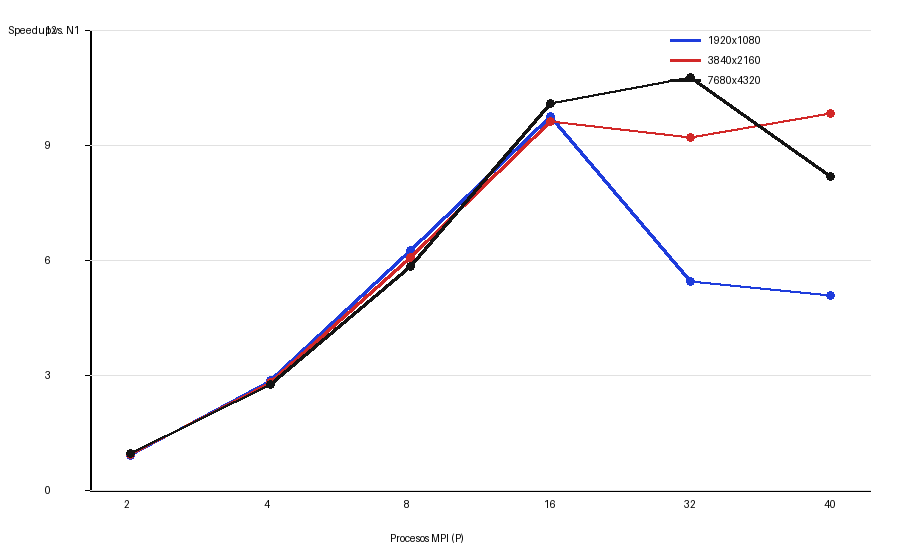
\includegraphics[width=.9\linewidth]{fig_speedup.png}
\caption{Speedup respecto a $T_1$ de N1 en funci\'on de $P$ (1 repetici\'on).}\label{fig:sp}
\end{figure}
\begin{figure}[t]
\centering
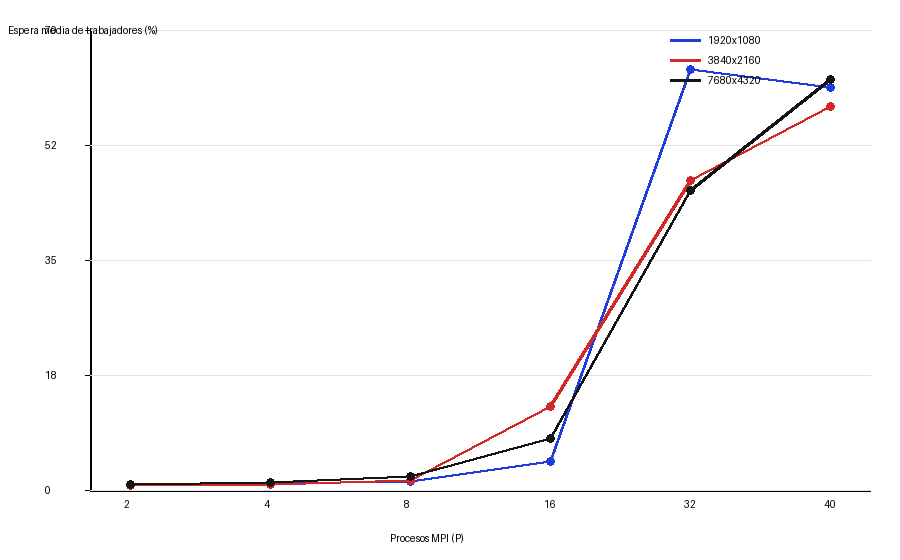
\includegraphics[width=.9\linewidth]{fig_espera.png}
\caption{Porcentaje medio de espera de los trabajadores en funci\'on de $P$.}\label{fig:es}
\end{figure}
\begin{figure}[t]
\centering

\includegraphics[width=\linewidth]{prueba1_1920x1080.png}
\caption{Imagen 1920$\times$1080 generada por el cl\'uster (ejecuci\'on con $P=40$).}\label{fig:img}
\end{figure}

\subsection{Prueba de sensibilidad con 5000 iteraciones}
Para cubrir el extremo superior del intervalo pedido (1k a 5k iteraciones) se repitió el barrido solo con las
pruebas 1 y 2, con una repetición. La Tabla~\ref{tab:5k} muestra los resultados; la prueba 3 no se repitió por
falta de tiempo.
\begin{table}[t]
\caption{Resultados con 5000 iteraciones (1 repetición). Mismo esquema que las tablas anteriores.}\label{tab:5k}
\centering\footnotesize
\begin{tabular}{|r|r|r|r|r|}\hline
$P$ & $T_P$ (s) & Speedup & Eficiencia & Espera \\ \hline
\multicolumn{5}{|l|}{\textit{1920$\times$1080, 2040 tareas}} \\ \hline
2 & 6.589 & 0.99 & 98.8\,\% & 0.3\,\% \\ \hline
4 & 2.309 & 2.82 & 94.0\,\% & 0.3\,\% \\ \hline
8 & 1.160 & 5.61 & 80.2\,\% & 0.4\,\% \\ \hline
16 & 0.737 & 8.84 & 58.9\,\% & 1.9\,\% \\ \hline
32 & 0.512 & 12.71 & 41.0\,\% & 27.0\,\% \\ \hline
40 & 0.464 & 14.03 & 36.0\,\% & 30.7\,\% \\ \hline
\multicolumn{5}{|l|}{\textit{3840$\times$2160, 8160 tareas}} \\ \hline
2 & 26.431 & 0.95 & 95.1\,\% & 0.3\,\% \\ \hline
4 & 9.634 & 2.61 & 86.9\,\% & 0.3\,\% \\ \hline
8 & 4.873 & 5.16 & 73.7\,\% & 0.4\,\% \\ \hline
16 & 2.966 & 8.47 & 56.5\,\% & 0.9\,\% \\ \hline
32 & 1.720 & 14.61 & 47.1\,\% & 16.1\,\% \\ \hline
40 & 1.696 & 14.81 & 38.0\,\% & 22.5\,\% \\ \hline
\end{tabular}
\end{table}


\section{Discusi\'on}
\textbf{Dentro de un nodo.} Hasta $P=8$ la eficiencia se mantiene entre 83\,\% y 95\,\% y la espera es menor a 2.1\,\%: el
maestro alcanza a alimentar a los trabajadores. Con $P=16$ la eficiencia baja a 64--67\,\% y el speedup se queda cerca de 10,
lo cual es consistente con que los 16 hilos de N1 son SMT sobre 8 n\'ucleos f\'isicos (el Ryzen 7 5700U tiene 8 n\'ucleos);
esta explicaci\'on no se verific\'o midiendo con SMT apagado.

\textbf{Entre nodos.} Al pasar a $P=32$ y $P=40$ la espera salta a 45--62\,\% en la prueba 3 y a 47--64\,\% en las
pruebas 1 y 2, y el tiempo deja de mejorar (en la prueba 3 empeora de 1.88\,s a 2.48\,s entre $P=32$ y $P=40$). Las causas
plausibles son (i) que el maestro, que recibe cada bloque por la red (RTT de 3\,ms) y atiende una cola de miles de tareas
peque\~nas, se convierte en cuello de botella, y (ii) que los trabajadores de N3, el nodo m\'as lento (su $T_1$ es de 1.9 a
2.4 veces el de N1), terminan tarde y dejan esperar al resto. Ninguna de las dos se aisl\'o con un experimento; son hip\'otesis.

\textbf{Efecto de las iteraciones.} Con 5000 iteraciones (Tabla~\ref{tab:5k}) el speedup con $P=40$ sube a 14.0 en 1080p y 14.8 en 4K,
y la espera baja a 31\,\% y 22\,\%, frente a 61\,\% y 58\,\% con 1000 iteraciones. Es consistente con que m\'as c\'omputo por tarea
amortiza el costo de repartir y recibir bloques; no se prob\'o ninguna otra causa.

\textbf{Resoluci\'on.} La prueba 1 (1080p) tiene pocas tareas y $T_P$ ya es de 0.12\,s con $P=16$, por lo que el
sobrecosto de comunicaci\'on pesa m\'as; las pruebas 2 y 3 retrasan la saturaci\'on, como se espera de un problema
con m\'as trabajo por proceso.

\section{Limitaciones}
\begin{itemize}
\item Una repetici\'on por configuraci\'on; las diferencias peque\~nas entre filas pueden ser ruido.
\item Entorno virtualizado (WSL2 en modo de red espejo) y laptops con planes de energ\'ia y t\'ermica distintos; el $T_1$ de
N2 (Ryzen 9) result\'o mayor que el de N1 pese a ser un CPU m\'as potente, sin que se haya investigado la causa.
\item El barrido llena N1 antes que N2 y N3 (\texttt{--map-by slot}), por lo que no se compar\'o un mismo $P$
repartido entre nodos con $P$ concentrado en uno.
\item Los \emph{slots} se fijaron al n\'umero de hilos l\'ogicos; no se prob\'o con n\'ucleos f\'isicos.
\end{itemize}

\section{Conclusiones}
El esquema maestro--trabajador con cola din\'amica de bloques de $32\times32$ produce la imagen correcta en las tres
resoluciones pedidas y escala con eficiencia alta dentro de un nodo. En este cl\'uster de tres laptops por Ethernet la
ganancia se estanca al cruzar nodos y el tiempo de espera de los trabajadores domina, por lo que, con estas mediciones,
el speedup m\'aximo respecto al nodo maestro fue de 10.8 con 1000 iteraciones y de 14.8 con 5000 iteraciones (prueba 2). Mejorar el reparto (tareas m\'as grandes, pre-asignaci\'on
ponderada por velocidad de nodo) y repetir las mediciones quedan como trabajo futuro.

\begin{thebibliography}{8}
\bibitem{mandelbrot} Mandelbrot, B.B.: Fractal aspects of the iteration of $z\mapsto\lambda z(1-z)$ for complex
$\lambda$ and $z$. Annals of the New York Academy of Sciences \textbf{357}, 249--259 (1980)
\bibitem{gropp} Gropp, W., Lusk, E., Skjellum, A.: Using MPI: Portable Parallel Programming with the
Message-Passing Interface. MIT Press (1999)
\end{thebibliography}
\end{document}
